%! Author = raphael
%! Date = 12/10/24

% Preamble
\documentclass[11pt]{article}

% Packages
\usepackage{amsmath}
\usepackage[a4paper, top=2cm, bottom=2cm, left=2cm, right=2cm]{geometry}
\usepackage{graphicx}
\usepackage{titlesec}
\usepackage{hyperref}

% Document
\begin{document}

\begin{titlepage}
    \begin{center}
        % Logos
        
\includegraphics[width=0.4\textwidth]{UM} \hfill{} % Replace with your first logo
        
\includegraphics[width=0.4\textwidth]{FDS} % Replace with your third logo

        \vspace{3cm}

        % Title with bars
        \hrulefill\\[0.4cm]
        {\Huge \textbf{Projet Bioinformatique : samReader}}\\[0.4cm]
        \hrulefill

        \vspace{1.5cm}

        \large{\textbf{Raphaël Ribes}}\\[0.5cm]

        \vfill

        % Horizontal image near the bottom
        https://github.com/RaphaelRibes/samReader
        \href{https://github.com/RaphaelRibes/samReader}{%
            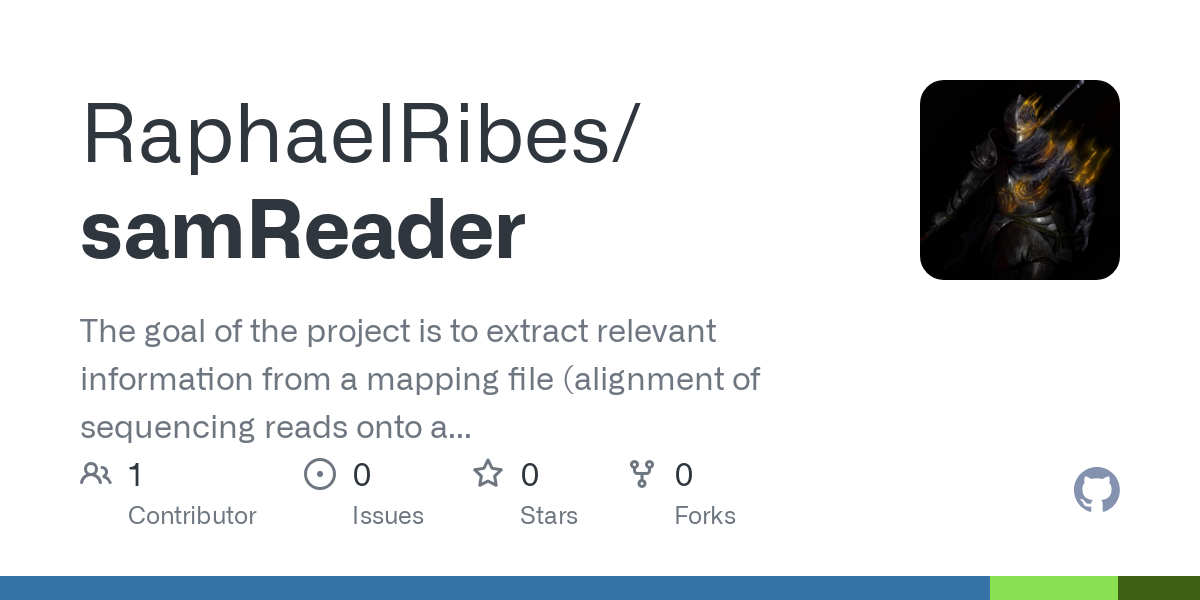
\includegraphics[width=0.8\textwidth]{samReader} % Replace with your horizontal image
        }
    \end{center}
\end{titlepage}

\section{Introduction}\label{sec:introduction}
Depuis l'émergence des technologies de séquençage de nouvelle génération (NGS), le volume et la complexité des données de séquences ADN ont augmenté de manière exponentielle.
Ces technologies, bien que révolutionnaires, génèrent des fragments courts de séquences ADN, appelés reads, qu'il est nécessaire d'aligner sur une séquence de référence pour les analyser efficacement.
Afin de standardiser et de faciliter le stockage et la manipulation de ces données d'alignement, le format SAM (Sequence Alignment/Map) a été introduit.
\\\\
\noindent Le format SAM offre une solution simple et flexible pour organiser les résultats d'alignement grâce à un fichier tabulé structuré, comprenant une section d'en-tête et une section de données d'alignement.
Ce format est indispensable pour des applications variées en biologie, allant de l'identification de mutations génétiques au suivi des populations écologiques.
Le fichier SAM permet également de traiter les reads correctement alignés, partiellement alignés ou mal alignés via des indicateurs (FLAGS) qui facilitent leur classification.

Ce Programme vise à lire, analyser et extraire les informations essentielles des fichiers SAM\@.
Le but est de faciliter l'interprétation des alignements, leur profondeur et leur qualité.
Cet outil permet une analyse des données issues des technologies de NGS plus simple et rapide.


\section{Présentation du format SAM}\label{sec:presentation-du-format-sam}


\section{Exemple d'application}\label{sec:exemple-d'application}


\section{Description du programme}\label{sec:description-du-programme}


\section{Discussion}\label{sec:discussion}
\textbf{Points forts}\label{subsec:points-forts}
\begin{itemize}
    \item \textbf{Rapports Résumés} : Génère des résumés complets des analyses sous forme de texte au format pdf.
    \item \textbf{Analyse Détaillée des Mutations} : Fournit des informations détaillées des mutations présentent sur les reads.
    \item \textbf{Analyse Spécifique aux Chromosomes} : Génère des répertoires distincts pour chaque chromosome, contenant les lectures alignées, partiellement alignées et non alignées.
    \item \textbf{Analyse de Profondeur} : Calcule la profondeur de couverture pour chaque chromosome.
    \item \textbf{Évolution de la Qualité d'Alignement} : Affiche l'évolution de la qualité d'alignement sur la longueur du chromosome.
    \item \textbf{Hautement Personnalisable} : Offre un large éventail d'options pour personnaliser l'analyse (voir comment utiliser \texttt{config.yaml}).
\end{itemize}

\noindent \textbf{Limitations}\label{subsec:points-faibles}
\begin{itemize}
    \item \textbf{Lenteur} : Le programme est lent.
    Trente pourcents de la durée d'exécution du programme est dû à la compilation des rapports ainsi qu'à la création des graphiques.
    \item \textbf{Interpolation sur des petits échantillons} : L'interpolation de la qualité d'alignement sur des petits échantillons peut être imprécise.
\end{itemize}

\end{document}